% PREAMBULE

% !BIB TS-program = biber
% !TEX TS-program = xelatexmk
% ITEX TS-program = latex

% !TEX spellcheck = French

\documentclass[class=article, crop=false]{standalone}
\usepackage[subpreambles=true]{standalone}
\usepackage{import}
\usepackage{blindtext}
\usepackage{fontspec}
\usepackage[french]{babel}
\usepackage{caption}
\usepackage{subcaption}
\usepackage{csquotes}
\usepackage{url}

%%%%%%%%%%%%%%%%%%%%%%%%
%			REFERENCES
% le package hyperref avec des options, si en local
\usepackage[pdfusetitle, pdfsubject ={Mémoire TNAH}, pdfkeywords={les mots-clés}]{hyperref}
\usepackage[backend=bibtex, sorting=nyt, style=verbose-ibid]{biblatex}
\addbibresource{../../../bib.bib}

%%%%%%%%%%%%%%%%%%%%%%%%
%			GLOSSAIRE
\usepackage[acronym]{glossaries}
\newglossaryentry{htr}
{
    name=Handwritten Text Recognition,
    description={La reconnaissance du texte écrit sur une image numérique}
}
\newacronym{HTR}{HTR}{Handwritten Text Recognition}

\newglossaryentry{ocr}
{
    name=Optical Character Recognition,
    description={La reconnaissance des polices du texte sur une image numérique}
}
\newacronym{OCR}{OCR}{Optical Character Recognition}

\newglossaryentry{Inria}
{
    name=Inria,
    description={Institut national de recherche en sciences et technologies du numérique}
}
\newacronym{INRIA}{Inria}{Institut national de recherche en sciences et technologies du numérique}

\newacronym{almanach}{ALMAnaCH}{Automatic Language Modelling and Analysis \& Computational Humanities}

\newglossaryentry{enc}
{
    name=École nationale des chartes,
    description={Grande école bla bla bla}
}
\newacronym{ENC}{ENC}{École nationale des chartes}

\newglossaryentry{HTR-United}
{
    name=HTR-United,
    description={HTR-United is a catalog and an ecosystem for sharing and finding ground truth for optical character or handwritten text recognition (OCR/HTR)}
}

\newglossaryentry{CLab}
{
	name=CREMMALab,
	description={Consortium pour la reconnaissance
d’'écriture manuscrite des matériaux anciens}
}
\newacronym{CREMMA}{CREMMA}{Consortium Reconnaissance
d’Écriture Manuscrite des Matériaux Anciens}

\newglossaryentry{tei}
{
	name={Text Encoding Initiative},
	description={Normes internationales de l'encodage des documents texts}
}
\newacronym{TEI}{TEI}{Text Encoding Initiative}

\newglossaryentry{iiif}
{
	name={International Image Interoperability Framework},
	description={Normes internationales de l'exploitation des images numériques et de leurs métadonnées par API}
}
\newacronym{IIIF}{IIIF}{International Image Interoperability Framework}

\newacronym{ALTO}{ALTO}{Analyzed Layout and Text Object}

\newacronym{XML}{XML}{eXtensible Markup Language}

\newacronym{BNF}{BnF}{Bibliothèque nationale de France}

\newacronym{RDF}{RDF}{Resource Description Framework}

\newacronym{TAL}{TAL}{Traitement automatique des langues}

\newacronym{ARK}{ARK}{Archival Resource Key}

\newacronym{DTS}{DTS}{Distributed Text Services}

\newglossaryentry{iiifapi}
{
	name={IIIF Image API},
	description={Un service de web qui renvoie une image suite à une requête standardisée HTTP(S). L'URI peut préciser la région, la taille, la rotation, la qualité, les caractéristiques, et le format de l'image demandée.}
}
\newacronym{API}{API}{Application Programming Interface}

\newglossaryentry{odd}
{
	name={One Document Does it all},
	description={Un fichier XML TEI qui précise les règles d'un schème TEI personnalisé.}
}
\newacronym{ODD}{ODD}{One Document Does it all}

\newacronym{JSON}{JSON}{JavaScript Object Notation}

\newacronym{HTML}{HTML}{HyperText Markup Language}

\newacronym{METS}{METS}{Metadata Encoding and Transmission Standard}

\newacronym{YAML}{YAML}{Yet Another Markup Language}

\newacronym{SRU}{SRU}{Search/Retrieve via URL}

\newglossaryentry{unimarc}
{
	name={UNIMARC},
	description={Une référence pour l’échange de données en format XML}
}

\newacronym{SUDOC}{SUDOC}{Système Universitaire de Documentation}

%%%%%%%%%%%%%%%%%%%%%%%%
%			DIAGRAM
\usepackage{tikz}
\usetikzlibrary{positioning}
\usetikzlibrary{calc, matrix, shapes.geometric, arrows}
\usepackage{pgfplots}
\usepackage{array}
\usepackage{tabularx}
\usepackage{graphicx}


%%%%%%%%%%%%%%%%%%%%%%%%
%			CODE
\usepackage{listings}
\usepackage{color}
\definecolor{codegray}{rgb}{0.5,0.5,0.5}
\definecolor{codepurple}{rgb}{0.58,0,0.82}
\definecolor{cyan}{rgb}{0.0,0.6,0.6}
\definecolor{codegreen}{rgb}{0,0.6,0}
\definecolor{backcolour}{rgb}{0.95,0.95,0.92}

\lstdefinelanguage{XML}{
  backgroundcolor=\color{backcolour},  
  basicstyle=\ttfamily\footnotesize,
  morestring=[s]{"}{"},
  moredelim=[s][\color{black}]{>}{<},
  morecomment=[s]{!--}{--},
  commentstyle=\color{codegreen},
  moredelim=[s][\color{red}]{\ }{=},
  stringstyle=\color{blue},
  identifierstyle=\color{cyan},
  numberstyle=\tiny\color{codegray},
  breakatwhitespace=false,         
    breaklines=true,                 
    captionpos=b,                    
    keepspaces=true,                 
    numbers=left,                    
    numbersep=5pt,                  
    showspaces=false,                
    showstringspaces=false,
    showtabs=false,                  
    tabsize=2
}

%Code listing style named "json"
\lstdefinestyle{json}{
  backgroundcolor=\color{backcolour}, 
  basicstyle=\ttfamily\footnotesize,
  commentstyle=\color{codegreen},
  numberstyle=\tiny\color{codegray},
  basicstyle=\ttfamily\footnotesize,
  breakatwhitespace=false,         
  breaklines=true,                 
  captionpos=b,                    
  keepspaces=true,                 
  numbers=left,                    
  numbersep=5pt,                  
  showspaces=false,                
  showstringspaces=false,
  showtabs=false,                  
  tabsize=2
}

%Code listing style named "python"
\definecolor{codepurple}{rgb}{0.58,0,0.82}

\lstdefinestyle{python}{
    backgroundcolor=\color{backcolour},   
    commentstyle=\color{codegreen},
    keywordstyle=\color{magenta},
    numberstyle=\tiny\color{codegray},
    stringstyle=\color{codepurple},
    basicstyle=\ttfamily\footnotesize,
    breakatwhitespace=false,         
    breaklines=true,                 
    captionpos=b,                    
    keepspaces=true,                 
    numbers=left,                    
    numbersep=5pt,                  
    showspaces=false,                
    showstringspaces=false,
    showtabs=false,                  
    tabsize=2
}

%%%%%%%%%%%%%%%%%%%%%%%%
%%%%%%%%%%%%%%%%%%%%%%%%
%			DOCUMENT
%%%%%%%%%%%%%%%%%%%%%%%%
%%%%%%%%%%%%%%%%%%%%%%%%
\begin{document}
J'ai créé l'application \texttt{alto2tei} afin de compléter le pipeline du projet \textit{Gallic(orpor)a}. Pour résumer, la première étape du pipeline est la récupération des pages numérisées du document source. Ensuite il prédit le texte et la mise en page du fac-similé numérique en traitant chaque page avec les modèles \acrshort{HTR}. Les données produites par les modèles sont en format \acrshort{XML} \acrshort{ALTO}. Mais le pipeline veut présenter les données enrichies par les métadonnées et par l'analyse linguistique en format \acrshort{XML} \acrshort{TEI} puisque le schème \acrshort{TEI} est plus utilisé et il convient mieux à l'édition du texte que le schème \acrshort{ALTO}. Mon application \texttt{alto2tei} a complété le pipeline en construisant un document \acrshort{TEI} à partir des données des modèles \acrshort{HTR}.

Cependant, les données du text transcrit ne constituent pas tout ce qu'il faut pour construire un document \acrshort{TEI}. Il faut aussi des métadonnées qui s'encadrent dans l'élément \acrshort{TEI} \texttt{<teiHeader>}. L'application \texttt{alto2tei} a donc besoin de récupérer les métadonnées à partir des sources externes, qui contiennent des données autre que celles créées par le pipeline. Pour y parvenir, l'application s'appuie sur la technologie d'\acrshort{API} (\acrlong{API}) qui lui permet de poser des questions aux sources en ligne et de comprendre leur réponse.

Quelles métadonnées faut-il chercher~? Dans le chapitre~\ref{chap:metadata}, je parle de trois objets de texte conceptuels pertinents~:  (1) la ressource numérique elle-même en format \acrshort{XML} \acrshort{TEI}, (2) le fac-similé numérique disponible depuis l'\acrshort{API} de la \acrshort{BNF} dont les images sont traités par les modèles \acrshort{HTR}, et (3) le document physique qui est conservé par la \acrshort{BNF} et qui a été numérisé. Chacun est distinct et ses métadonnées se trouvent depuis des sources différentes. Afin d'informer des métadonnées de la ressource numérique, il faut donc s'appuyer sur les métadonnées de ses trois objets de texte.

Le pipeline du projet \textit{Gallic(orpor)a} a besoin de diversifier sa manière de récupérer des métadonnées. L'application \texttt{alto2tei} profite de quatre sources externes de données afin de renseigner sur les trois documents conceptuels concernés.
\begin{enumerate}
\item les métadonnées sur la ressource lexicographique numérique
\begin{itemize}
\item source~: fichier de configuration personnalisable
\item format~: \acrshort{YAML} (\textit{\acrlong{YAML}})
\item portée~: informations administratives portant sur la création de la ressource, y compris les droits d'utilisation et les autorités qui s'en chargent
\end{itemize}
\item les métadonnées sur le fac-similé numérique
\begin{itemize}
\item source~: manifest \acrshort{IIIF} renvoyé de l'\acrshort{IIIF} \acrshort{API}
\item format~: \acrshort{JSON} (\textit{\acrlong{JSON}})
\item portée~: données bibliographiques qui servent à identifier les exemplaires numériques traités par des modèles \acrshort{HTR}
\end{itemize}
\item les métadonnées sur le document source physique
\begin{itemize}
\item source~: réponse à la requête envoyée à l'\acrshort{API} \acrshort{SRU} (\textit{\acrlong{SRU}}) de la \acrshort{BNF}, qui interroge le catalogue général de la \acrshort{BNF}
\item format~: \Gls{unimarc} \acrshort{XML}
\item portée~: données bibliographiques, y compris la responsabilité du document source, sa création, et sa conservation actuelle
\end{itemize}
\end{enumerate}
Les métadonnées sur le document source physique s'appuient encore sur une autre source de données afin de récupérer où se trouve l'institution qui héberge le document. Dans le cadre du projet \textit{Gallic(orpor)a}, la réponse à cette question est toujours Paris, puisque la \acrshort{BNF} se situe au capital. Mais, afin d'éviter l'encodage dur, l'application \texttt{alto2tei} recherche cette donnée dans la base de données du \acrlong{SUDOC} (\acrshort{SUDOC}) puisque la localisation de l'institution hôte du document physique n'est pas encodée dans les données \Gls{unimarc} selon l'usage de la \acrshort{BNF}.

\section{La récupération des métadonnées}
Comme s'explique dans le chapitre~\ref{chap:pipeline}, l'application \texttt{alto2tei} s'appuie sur un système de fichier fixé. Cela lui permet d'accéder à l'identifiant \acrshort{ARK} (\acrlong{ARK}) du document dont les pages numérisées ont été traitées par les modèles \acrshort{HTR}. Cet identifiant donne la clef aux données sur le fac-similé numérique encodées dans le \textit{manifest} \acrshort{IIIF} (\acrlong{IIIF}). L'une des données dans le \textit{manifest} \acrshort{IIIF}, au moins pour les documents de la base de données Gallica, porte sur la relation entre le fac-similé numérique est la source physique à partir duquel le fac-similé numérique a été produit. (cf.~Fig.~\ref{fig:relation}) Cette relation permet de rechercher les métadonnées du document physique dans le catalogue général de la \acrshort{BNF}.

\begin{figure}[ht]
\centering
\lstset{style=json}
\begin{lstlisting}[language=Python]
"metadata": [
	{
	"label": "Relation",
	"value": "Notice du catalogue : http://catalogue.bnf.fr/ark:/12148/cb30369299r"
	},
]
\end{lstlisting}
\caption{Une partie du \textit{manifest} \acrshort{IIIF} pour le fac-similé numérique d'\acrshort{ARK} \texttt{bpt6k1281160s}, un imprimé numérisé sur Gallica}
\label{fig:relation}
\end{figure}

Si la relation entre le document numérique sur Gallica et le document physique dans l'un des magasin des la \acrshort{BNF} n'est pas établie, l'application \texttt{alto2tei} n'abandonne pas tout essai de produire un document \acrshort{TEI}. Au lieu de s'arrêter, elle compte uniquement sur les données du \textit{manifest} \acrshort{IIIF}. Ces données sont vérifiées puisqu'elles portent sur le fac-similé numérique dont les images les modèles \acrshort{HTR} du pipeline ont traité. Le fac-similé numérique est toujours l'un des objets de texte pertinents aux métadonnées de la ressource. L'application \texttt{alto2tei} peut donc créer deux genres de \texttt{<teiHeader>}, l'un avec un maximum d'information et l'autre, au cas où la relation entre le fac-similé numérique et le document physique n'était pas établie, avec un peu moins d'information.

En tout cas, chaque genre de \texttt{<teiHeader>} aura la même arborescence parce que tout élément est d'abord créé avec des données par défaut, telle que la phrase \og{}\textit{Information not available}\fg{}. La donnée par défaut est ensuite remplacée par la donnée récupérée des sources externes. Par conséquent, l'application \texttt{alto2tei} ne s'arrête pas si une donnée n'est pas récupérée. Il peut arriver, par exemple, que la relation entre le document physique et le fac-similé numérique est établie et les données du catalogue sont traitées, mais une donnée en particulière n'est pas disponible dans la notice du document physique. Dans ce cas, le \texttt{<teiHeader>} aura des éléments qui contiennent une phrase par défaut même si des autres éléments contiennent des données récupérées depuis la source ciblée. L'application \texttt{alto2tei} essaie de fournir autant des métadonnées que possible et surmonter les particularités de la disponibilité des données.

\section{Les sources des métadonnées}
Quatre source de données servent à informer des éléments du \texttt{<teiHeader>}. Elles sont le \textit{manifest} \acrshort{IIIF}, les données \Gls{unimarc} du catalogue général de la \acrshort{BNF}, la base de données du site web du \acrlong{SUDOC} (\acrshort{SUDOC}), le fichier de configuration, et les fichiers \acrshort{ALTO} produits par des modèles \acrshort{HTR}. Les trois premières sources exigent une requête au bon \acrshort{API}. Le \textit{manifest} \acrshort{IIIF} est renvoyé par une requête à l'\acrshort{API} \acrshort{IIIF} du fac-similé numérique sur Gallica, selon les normes imposées par la \acrshort{BNF}. Les données \Gls{unimarc} du catalogue général de la \acrshort{BNF} sont accessible à partir d'une requête à l'\acrshort{API} \acrshort{SRU} (\textit{\acrlong{SRU}} de la \acrshort{BNF}. Enfin, les données du \acrlong{SUDOC} sont renvoyées à partir d'une requête à l'\textit{endpoint} \acrshort{API} du site \acrshort{SUDOC}. L'application \texttt{alto2tei} se dispose directement du fichier de configuration et des fichiers \acrshort{ALTO} qu'elle traite.

\subsection{Le format du \textit{manifest} \acrshort{IIIF}}
Le \textit{manifest} \acrshort{IIIF} est un format de données standardisés qui est envoyé par tout \acrshort{API} \acrshort{IIIF} selon le syntaxe de requête demandé par l'organisation qui gère l'\acrshort{API}. La \acrlong{BNF} exige le syntaxe suivant pour toute requête envoyée à l'\acrshort{API} \acrshort{IIIF} des fac-similés numériques sur Gallica~:
\begin{verbatim}
https://gallica.bnf.fr/iiif/ark:/12148/<ARK>/manifest.json
\end{verbatim}
Pour utiliser cette requête, il faut simplement remplacer la partie \texttt{<ARK>} par l'\acrshort{ARK} du document cherché. Grâce au système de fichier du pipeline \textit{Gallic(orpor)a}, l'\acrshort{ARK} du document est facilement disponible. Il est le nom du dossier qui contient les fichiers \acrshort{ALTO} traités.

La structure du \textit{manifest} \acrshort{IIIF} peut varier un peu, mais certains composants sont toujours attendus. Le Tableau~\ref{tab:manifestExample} montre toute clef principale du \textit{manfiest} pour un fac-similé numérique mis en ligne sur Gallica par la \acrshort{BNF}. L'exemple prend le livret imprimé du ballet \textit{Les divers entretiens de la fontaine de Vaucluse} de 1649, dont le fac-similé a l'identifiant \texttt{bpt6k1513919s}. Les parties les plus importants sont aussi les plus complexes, la clef \textit{metadata} et la clef \textit{sequences}. La première contient une suite des pairs clef-valeur, chacun porte sur une métadonnée du fac-simlié numérique. La dernière s'appuie sur les images numériques. Pour l'application \texttt{alto2tei} et la création du \texttt{<teiHeader>} les métadonnées du \textit{manifest} sont l'essentiel.

\begin{figure}[htp]
\begin{tabularx}{\textwidth}{ 
  | m{5em}
  | >{\arraybackslash}X 
  |}
\hline
\textbf{clef} & \textbf{valeur}\\
\hline \hline
@id & https://gallica.bnf.fr/iiif/ark:/12148/bpt6k1513919s/manifest.json\\
\hline
label & BnF, département Réserve des livres rares, RES-YF-1990\\
\hline
attribution & Bibliothèque nationale de France\\
\hline
license & https://gallica.bnf.fr/html/und/conditions-dutilisation-des-contenus-de-gallica\\
\hline
logo & https://gallica.bnf.fr/mbImage/logos/logo-bnf.png\\
\hline
related & https://gallica.bnf.fr/ark:/12148/bpt6k1513919s\\
\hline
description & Les divers entretiens de la fontaine de Vaucluse : ballet dansé à la grande salle du Roure l'année 1649...\\
\hline
metadata & \textit{suite des pairs qui portent sur les métadonnées du fac-similé numérique}\\
\hline
sequences & \textit{imbrication complexe pour contenir des données sur les images, dit canvases, du fac-similé numérique}\\
\hline
thumbnail & \textit{pair qui contient un lien pour l'aperçu du document}\\
\hline
context & http://iiif.io/api/presentation/2/context.json\\
\hline
\end{tabularx}

\caption{Les clefs principales du \textit{manifest} \acrshort{IIIF} d'un document sur Gallica (\acrshort{ARK} \texttt{bpt6k1513919s})}
\label{tab:manifestExample}
\end{figure}

Le contenu du \textit{metadata} du \textit{manifest} \acrshort{IIIF} peut varier de document à document, même quand les données sont encodées par la même institution telle que la \acrlong{BNF}. Comme s'explique dans le chapitre~\ref{chap:metadata}, il faut déterminer l'essentiel quant aux métadonnées à mettre dans le schème \acrshort{TEI}. Il faut chercher les métadonnées qui s'appliquent tous les deux aux manuscrits et aux imprimés. En plus de cela, il faut aussi chercher les métadonnées qui, selon l'usage de la \acrshort{BNF}, sont normalement encodées dans le \textit{manifest} \acrshort{IIIF} du document sur Gallica. J'ai déterminé que l'essentiel du \textit{manifest} \acrshort{IIIF} sont les métadonnées listée dans le Tableau~\ref{tab:metadataManfiest}.

\begin{figure}[htp]
\begin{tabularx}{\textwidth}{ 
  | m{5em}
  | >{\arraybackslash}X 
  |}
\hline
\textbf{\textit{label}} & \textbf{\textit{value}}\\
\hline \hline
Relation & Notice du catalogue : http://catalogue.bnf.fr/ark:/12148/cb33352789b \\ \hline
Repository & Bibliothèque nationale de France\\ \hline
Shelfmark & Bibliothèque nationale de France, département Réserve des livres rares, RES-YF-1990\\ \hline
Title & Les divers entretiens de la fontaine de Vaucluse~: ballet dansé à la grande salle du Roure l'année 1649\\ \hline
Language & français\\ \hline
Creator & Nouguier, de. Auteur du texte\\ \hline
Date & 1649\\ \hline
\end{tabularx}
\caption{Les métadonnées essentielles du \textit{manifest} \acrshort{IIIF} (\acrshort{ARK} \texttt{bpt6k1513919s})}
\label{tab:metadataManfiest}
\end{figure}

Certaines métadonnées du \textit{manifest} posent des avantages et des défis. L'un des avantages est la manière par laquelle la \acrshort{BNF} encode la donnée \textit{Relation} pour les documents mis sur Gallica. La donnée \textit{Relation} peut se répéter parce que le fac-similé peut être lié aux plusieurs notices du catalogue. Cependant, elle termine toujours par l'\acrshort{ARK} unique du document physique auquel le fac-similé est lié. Ainsi, l'application \texttt{alto2tei} se dispose de la donnée \textit{Relation} et, en traitant la fin de la chaîne, extrait l'\acrshort{ARK} du document physique dans le catalogue général de la \acrshort{BNF}. Un défi à surmonter est quand un type (\textit{label}) de métadonnée n'est pas répété mais il contient plusieurs valeurs. Cela peut arriver quand un document a plusieurs auteurs. Pour cette raison, l'application \texttt{alto2tei} traite l'encodage de toute donnée sur l'auteur d'une manière différente que les autres métadonnées.

\subsection{Le format \Gls{unimarc}}
Étant communiquées en \acrshort{XML}, les données du catalogue général de la \acrshort{BNF} se trouvent sur l'arbre de la notice en format \Gls{unimarc}~; ce format leur donne le préfix \texttt{mxc} qui fait référence au \textit{MarcXchange}. Un exemple des données \Gls{unimarc} renvoyées par l'\acrshort{API} \acrshort{SRU} de la \acrshort{BNF} est montré dans la Figure~\ref{fig:unimarc}. L'exemple prend toujours le livret imprimé du ballet \textit{Les divers entretiens de la fontaine de Vaucluse} de 1649. Le fac-similé numérique sur Gallica a l'identifiant \texttt{bpt6k1513919s}. Mais, comme expliqué ci-dessus, l'identifiant du document physique est récupéré en examinant le \textit{manifest} \acrshort{IIIF} du fac-similé numérique. L'\acrshort{ARK} du document physique (\texttt{cb33352789b} dans l'exemple) permet d'interroger les données du catalogue général de la \acrshort{BNF} grâce à son \acrshort{API} \textit{\acrlong{SRU}} (\acrshort{SRU}).

\begin{figure}[ht]

\begin{subfigure}[b]{\textwidth}
\lstset{style=python}
\begin{lstlisting}[language=python]
class SRU:
	def __init__(self, ark):
		"""Args: 
			ark (string): document ARK in BnF catalogue"""
		self.ark = ark
		
	def request(self):
		r = requests.get(f'http://catalogue.bnf.fr/api/SRU?version=1.2&operation=searchRetrieve&query=(bib.persistentid all "ark:/12148/{self.ark}")')
\end{lstlisting}
\caption{La requête envoyée à l'\acrshort{API} \acrshort{SRU} par l'application python \texttt{alto2tei}}
\label{fig:sruRequest}
\end{subfigure}

\begin{subfigure}[b]{\textwidth}
\begin{lstlisting}[language=XML]
<srw:searchRetrieveResponse xmlns:srw="http://www.loc.gov/zing/srw/" xmlns="http://catalogue.bnf.fr/namespaces/InterXMarc">
<!-- ... -->
	<srw:echoedSearchRetrieveRequest>
		<srw:query>(bib.persistentid all "ark:/12148/cb33352789b")</srw:query>
	</srw:echoedSearchRetrieveRequest>
	<srw:numberOfRecords>1</srw:numberOfRecords>
	<srw:records>
		<srw:record>
			<srw:recordSchema>marcxchange</srw:recordSchema>
			<srw:recordPacking>xml</srw:recordPacking>
			<srw:recordData>
				<mxc:record format="Unimarc" id="ark:/12148/cb33352789b" type="Bibliographic" xmlns:mxc="info:lc/xmlns/marcxchange-v2">
<!-- data in Unimarc formatting, with prefix "mxc" -->
				</mxc:record>
			</srw:record>
		</srw:recordData>
<!-- ... -->
\end{lstlisting}
\caption{La réponse de l'\acrshort{API} \acrshort{SRU} pour le document d'\acrshort{ARK} \texttt{bpt6k1513919s}}
\label{fig:unimarc}
\end{subfigure}

\caption{La requête et la réponse à l'API SRU [version 1.2]}
\end{figure}

Les données \Gls{unimarc} sont emballées dans les éléments du préfix \texttt{srw} qui fait référence au protocole \acrshort{SRU}.\footcite{SRUSearchRetrieval} L'élément \texttt{<srw:recordData>} (ligne 11, Fig~\ref{fig:unimarc}) présente les données da la notice du catalogue trouvée. L'application \texttt{alto2tei} détermine qu'elle a bien localisé le bon document physique dans le catalogue de la \acrshort{BNF} si la réponse de l'\acrshort{API} \acrshort{SRU} ne contient qu'une seule notice. Le nombre de notices trouvées est sur la ligne 6 de la Figure~\ref{fig:unimarc}. Si ce nombre est plus que \og{}1\fg{} cela indique que l'\acrshort{ARK} récupéré de la donnée \textit{Relation} du \textit{manifest} \acrshort{IIIF} est lié aux notices de plusieurs documents. Ne pouvant pas déterminer quel document est le bon, l'application \texttt{alto2tei} abandonne les données \Gls{unimarc} et compte uniquement sur les métadonnées du \textit{manifest} \acrshort{IIIF}.

\subsection{Le format du fichier de configuration}

\subsection{Le format des données du site \acrshort{SUDOC}}


\section{La mise en place des données récupérées}
Ayant découvert les formats de données des quatre sources de données utilisées pour remplir le \texttt{<teiHeader>}, il faut parler d'où ses données ainsi récupérées vont.

\subsection{Les sources des données du \texttt{<titleStmt>}}
La Figure~\ref{fig:titleStmt} visualise les sources des données du \texttt{<titleStmt>}. Les éléments portant sur le titre de la ressource (\texttt{<title>}) et sur les personnes auxquels est attribuée la propriété intellectuelle du texte représenté (\texttt{<author>}) sont informés par l'un de deux sources de données possible. Soit les données du catalogue général donnent beaucoup d'information sur les auteurs ainsi qu'un titre propre, soit le \textit{manifest} \acrshort{IIIF} donne le titre du texte et les noms non annotés des auteurs. Le choix entre les deux sources de données se fait à partir de la disponibilité des données du catalogue de la \acrshort{BNF}. D'habitude, l'application \texttt{alto2tei} met en priorité les données du catalogue. Les éléments descendants du \texttt{<respStmt>} s'appuient toujours sur le fichier de configuration afin qu'ils puissent être personnalisés par les personnes qui utilisent l'application \texttt{alto2tei} pour générer leurs propres documents \acrshort{TEI}.

\tikzstyle{iiif} = [rectangle, rounded corners, minimum width=2cm, minimum height=0.5cm, text centered, draw=black, fill=blue!30]
\tikzstyle{both} = [rectangle, rounded corners, minimum width=2cm, minimum height=0.5cm, text centered, draw=black, fill=violet!30]
\tikzstyle{unimarc} = [rectangle, rounded corners, minimum width=2cm, minimum height=0.50cm, text centered, draw=black, fill=red!30]
\tikzstyle{config} = [rectangle, rounded corners, minimum width=2cm, minimum height=0.5cm, text centered, draw=black, fill=green!30]
\tikzstyle{sudoc} = [rectangle, rounded corners, minimum width=2cm, minimum height=0.5cm, text centered, draw=black, fill=yellow!30]
\tikzstyle{files} = [rectangle, rounded corners, minimum width=2cm, minimum height=0.5cm, text centered, draw=black, fill=gray!30]
\tikzstyle{elem} = [rectangle, rounded corners, minimum width=2cm, minimum height=0.5cm, text centered, draw=black]
\tikzstyle{arrow} = [thick,>=stealth]
\tikzset{line/.style={draw, thick, -latex'}}

\begin{figure}[htp]
\centering
% legend
\begin{subfigure}[b]{0.4\textwidth}
\begin{tikzpicture}
\matrix [draw] {
	\node [iiif,label=right:manifest IIIF] {};\\
	\node [unimarc,label=right:Unimarc] {};\\
	\node [config,label=right:fichier de config] {}; \\
	\node [sudoc,label=right:SUDOC] {}; \\
	\node [files,label=right:fichiers traités] {}; \\
};
\end{tikzpicture}
\end{subfigure}

\vspace{1cm}


% <author> with relation
\begin{subfigure}[b]{0.7\textwidth}
\begin{tikzpicture}[node distance=0.5cm]

\node [elem] (titleStmt) {titleStmt};
\node [unimarc, right=of titleStmt] (title) {title};
\node [elem, below=of title] (author) {author};
\node [elem, right=of author] (persName) {persName};
\node [unimarc, right=of persName] (forename) {forename};
\node [unimarc, below=of forename] (surname) {surname};
\node [unimarc, below=of surname] (ptr) {ptr};

\draw [arrow] (titleStmt) -- (title);
\draw [arrow]
	(author) -| node[pos=0.25] {} (titleStmt);
\draw [arrow] (author) -- (persName);
\draw [arrow] (persName) -- (forename);
\draw [arrow]
	(surname) -| node[pos=0.25] {} (persName);
\draw [arrow]
	(ptr) -| node[pos=0.25] {} (persName);

\end{tikzpicture}
\caption{Les sources de données du \texttt{<title>} et du \texttt{<author>} quand la relation entre le fac-similé numérique et le document physique est établie}
\label{fig:sourceAuthor}
\end{subfigure}

\vspace{1cm}

% <author> without relation
\begin{subfigure}[b]{0.7\textwidth}
\begin{tikzpicture}[node distance=0.5cm]

\node [elem] (titleStmt) {titleStmt};
\node [iiif, right=of titleStmt] (title) {title};
\node [elem, below=of title] (author) {author};
\node [elem, right=of author] (persName) {persName};
\node [iiif, right=of persName] (name) {name};

\draw [arrow] (titleStmt) -- (title);
\draw [arrow]
	(author) -| node[pos=0.25] {} (titleStmt);
\draw [arrow] (author) -- (persName);
\draw [arrow] (persName) -- (forename);
\draw [arrow] (persName) -- (name);

\end{tikzpicture}
\caption{Les sources de données du \texttt{<title>} et du \texttt{<author>} quand la relation entre le fac-similé numérique et le document physique \textit{n'est pas} établie}
\label{fig:sourceAuthorWO}
\end{subfigure}

\vspace{1cm}

% <respStmt>
\begin{subfigure}[b]{0.7\textwidth}
\begin{tikzpicture}[node distance=0.5cm]

\node [elem] (titleStmt) {titleStmt};
\node [elem, right=of titleStmt] (respStmt) {respStmt};
\node [config, right=of respStmt] (resp) {resp};
\node [elem, right=of respStmt, below=of resp] (persName) {persName};
\node [config, right=of persName] (forename) {forename};
\node [config, below=of forename] (surname) {surname};
\node [config, below=of surname] (ptr) {ptr};

\draw [arrow] (titleStmt) -- (respStmt);
\draw [arrow] (respStmt) -- (resp);
\draw [arrow] 
	(persName) -| node[pos=0.25] {} (respStmt);
\draw [arrow] (persName) -- (forename);
\draw [arrow]
	(surname) -| node[pos=0.25] {} (persName);
\draw [arrow]
	(ptr) -| node[pos=0.25] {} (persName);
	
\end{tikzpicture}
\caption{Les sources de données du \texttt{<respStmt>} dans tout cas}
\label{fig:titleStmt}
\end{subfigure}

\vspace{1cm}

\caption{Les sources de données des éléments du \texttt{<titleStmt>}}
\label{fig:titleStmt}
\end{figure}

La Figure~\ref{fig:sourceAuthor} visualise les éléments du \texttt{<titleStmt>} dans le cas où la relation entre le fac-similé numérique sur Gallica et le document physique appartenant à la \acrshort{BNF} est établie. Cela veut dire que le document dont parle la notice du catalogue est le même document à partir duquel le fac-similé numérique sur Gallica a été fait. Quand la notice du bon document est trouvée, les données \Gls{unimarc} cherchées depuis le catalogue sont (1) le titre uniforme du document et (2) le nom et l'identifiant de ses auteurs.


\subsection{Les sources des données du \texttt{<extent>}}
L'élément \texttt{<extent>} du \texttt{<teiHeader>}, qui indique le nombre de fichiers traités par l'application \texttt{alto2tei} lors de la création de la ressource numérique, s'appuie simplement sur un compte des fichiers. L'application a besoin de traiter tout fichier \acrshort{ALTO} dans le dossier du document, expliqué dans la section~\ref{structure-fichier}, et mettre ses données dans le \texttt{<sourceDoc>}, selon la modélisation de l'application \texttt{alto2tei}. Elle peut également compter le nombre des fichiers \acrshort{ALTO} qui appartiennent au document. Ce compte elle met comme la \og{}taille\fg{} de la ressource numérique, dans l'élément \texttt{<measure>}.

\begin{figure}[htp]
\centering
\begin{tikzpicture}[node distance=0.5cm]

\matrix [draw,above=of start] {
	\node [iiif,label=right:manifest IIIF] {};\\
	\node [both,label=right:IIIF ou Unimarc] {}; \\
	\node [unimarc,label=right:données Unimarc] {};\\
	\node [config,label=right:fichier de config] {}; \\
	\node [sudoc,label=right:SUDOC] {}; \\
	\node [files,label=right:fichiers traités] {}; \\
};

\node [elem] (start) {extent};
\node [files, right=of start] (measure) {measure};

\draw [arrow]
	(start) -- (measure);

\end{tikzpicture}
\caption{}
\label{fig:dataExtent}
\end{figure}

\subsection{Les sources des données du \texttt{<publicationStmt>}}
La distribution de la ressource numérique est décrite par l'élément \texttt{<publicationStmt>}. Cet élément peut compter uniquement--et idéalement--sur les données du catalogue général de la \acrshort{BNF} en format \Gls{unimarc}. Mais si l'application a besoin, elle peut remplir certains éléments du \texttt{<publicationStmt>} en laissant vide des autres puisque le \textit{manifest} \acrshort{IIIF} peut renseigner sur l'auteur du document, son titre, et sa date de création.

\begin{figure}[htp]
\centering
\begin{tikzpicture}[node distance=0.5cm]

\matrix [draw,above=of start] {
	\node [iiif,label=right:manifest IIIF] {};\\
	\node [both,label=right:IIIF ou Unimarc] {}; \\
	\node [unimarc,label=right:données Unimarc] {};\\
	\node [config,label=right:fichier de config] {}; \\
	\node [sudoc,label=right:SUDOC] {}; \\
	\node [files,label=right:fichiers traités] {}; \\
};



\end{tikzpicture}
\caption{}
\label{fig:dataPS}
\end{figure}

\subsection{Les sources des données du \texttt{<sourceDesc>}}

\begin{figure}[htp]
\centering
\begin{tikzpicture}[node distance=0.5cm]



\end{tikzpicture}
\caption{}
\label{fig:dataSD}
\end{figure}

\subsection{Les sources des données du \texttt{<profileDesc>}}

\begin{figure}[htp]
\centering
\begin{tikzpicture}[node distance=0.5cm]



\end{tikzpicture}
\caption{}
\label{fig:dataPS}
\end{figure}

\subsection{Les sources des données du \texttt{<encodingDesc>}}

\begin{figure}[htp]
\centering
\begin{tikzpicture}[node distance=0.5cm]



\end{tikzpicture}
\caption{}
\label{fig:dataED}
\end{figure}



Parler de la récupération des données depuis les deux APIs discutés (cf.\,fig.~\ref{fig:workflow}) ainsi que le fichier YAML de configuration.

\begin{figure}
\centering
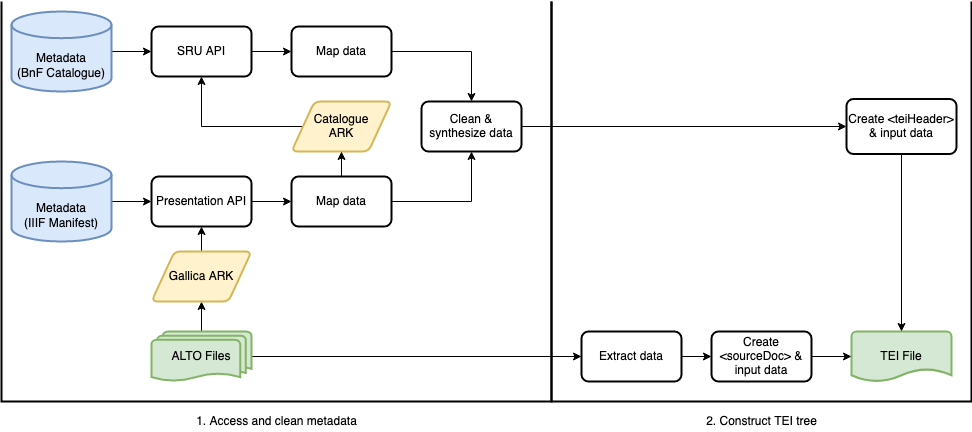
\includegraphics[width=\textwidth]{../../../images/full_tree.png}
\label{fig:workflow}
\caption{Workflow}
\end{figure}

\subsection{Du manifest IIIF à un dictionnaire Python}

Montrer le mapping des données du manifest au dictionnaire Python.

\subsection{De l'Unimarc à un dictionnaire Python}

Montrer le mapping des données du catalogue au dictionnaire Python.

\section{L'analyse des données}

Parler de la stratégie d'atténuation des risques en sélectionnant les données fiables. Les métadonnées du catalogue général de la BnF sont utilisées uniquement si le même exemplaire physique du document numérisé sur Gallica a bien été trouvé. Sinon, on risque de mettre les données d'un autre exemplaire de l'oeuvre que celui qui a été transcrit et donc introduire des fausses données, tel que le cote ou même l'éditeur et la date de publication de l'exemplaire.

\section{Le modèle du \texttt{<teiHeader>}}

Montrer le mapping des données au \texttt{<teiHeader>}.

\end{document}
\documentclass[../main.tex]{subfiles}